\documentclass[compress]{beamer}
\usepackage{ifthen,verbatim,hyperref}

\newcommand{\isnote}{}
\xdefinecolor{lightyellow}{rgb}{1.,1.,0.25}
\xdefinecolor{darkblue}{rgb}{0.1,0.1,0.7}

%% Uncomment this to get annotations
%% \def\notes{\addtocounter{page}{-1}
%%            \renewcommand{\isnote}{*}
%% 	   \beamertemplateshadingbackground{lightyellow}{white}
%%            \begin{frame}
%%            \frametitle{Notes for the previous page (page \insertpagenumber)}
%%            \itemize}
%% \def\endnotes{\enditemize
%% 	      \end{frame}
%%               \beamertemplateshadingbackground{white}{white}
%%               \renewcommand{\isnote}{}}

%% Uncomment this to not get annotations
\def\notes{\comment}
\def\endnotes{\endcomment}

\setbeamertemplate{navigation symbols}{}
\setbeamertemplate{headline}{\mbox{ } \hfill
\begin{minipage}{5.5 cm}
\vspace{-0.75 cm} \small
\end{minipage} \hfill
\begin{minipage}{4.5 cm}
\vspace{-0.75 cm} \small
\begin{flushright}
\ifthenelse{\equal{\insertpagenumber}{1}}{}{Jim Pivarski \hspace{0.2 cm} \insertpagenumber\isnote/\pageref{numpages}}
\end{flushright}
\end{minipage}\mbox{\hspace{0.2 cm}}\includegraphics[height=1 cm]{../cmslogo} \hspace{0.1 cm} \includegraphics[height=1 cm]{../tamulogo} \hspace{0.01 cm} \vspace{-1.05 cm}}

\begin{document}
\begin{frame}
\vfill
\begin{center}
\textcolor{darkblue}{\Large Monitoring of Alignment Triggers}

\vfill
\begin{columns}
\column{0.3\linewidth}
\begin{center}
\large
\textcolor{darkblue}{Jim Pivarski}
\end{center}
\end{columns}

\begin{columns}
\column{0.3\linewidth}
\begin{center}
\scriptsize
{\it Texas A\&M University}
\end{center}
\end{columns}

\vfill
 2 February, 2009

\end{center}
\end{frame}

%% \begin{notes}
%% \item This is the annotated version of my talk.
%% \item If you want the version that I am presenting, download the one
%% labeled ``slides'' on Indico (or just ignore these yellow pages).
%% \item The annotated version is provided for extra detail and a written
%% record of comments that I intend to make orally.
%% \item Yellow notes refer to the content on the {\it previous} page.
%% \item All other slides are identical for the two versions.
%% \end{notes}

\small

\begin{frame}
\frametitle{Status of alignment triggers (1/3)}

\vfill
As an overview, I'll summarize the status of all alignment-related triggers and their monitoring

\vfill
\begin{itemize}\setlength{\itemsep}{0.5 cm}
\item \textcolor{darkblue}{Muon triggers} {\scriptsize (HLT\_Mu5, HLT\_Mu9, HLT\_Mu11, \ldots)}
\begin{itemize}
\item primary triggers for long-term alignment \mbox{(tracker and muon systems)\hspace{-1 cm}}
\item \textcolor{darkblue}{status:} covered by muon physics groups
\end{itemize}

\item \textcolor{darkblue}{Muon beam-halo} {\scriptsize (HLT\_CSCBeamHalo, HLT\_CSCBeamHaloRing2or3, HLT\_CSCBeamHaloOverlapsRing1, HLT\_CSCBeamHaloOverlapsRing2)}
\begin{itemize}
\item \textcolor{darkblue}{what it is:} CSC trigger with a different $\eta$ cut in L1, \\ \textcolor{white}{what it is:} CSC RecHit pattern requirements in HLT
\item \textcolor{darkblue}{why we need it:} align muon endcaps earlier and more quickly
\item \textcolor{darkblue}{status:}
\begin{itemize}
\item L1 hardware and emulator are working, HLT paths exist
\item L1 data are being monitored
\item need to expand monitoring to HLT paths and \mbox{release validation\hspace{-1 cm}}
\item responsible: Joseph Gartner (U.\ Florida)
\end{itemize}
\end{itemize}

\end{itemize}
%% \hspace{-0.83 cm} \textcolor{darkblue}{\Large Outline2}
\end{frame}

\begin{frame}
\frametitle{Status of alignment triggers (2/3)}
\begin{itemize}\setlength{\itemsep}{0.25 cm}
\item \textcolor{darkblue}{Tracker-pointing cosmics} {\scriptsize (HLT\_TrackerCosmics)}
\begin{itemize}
\item \textcolor{darkblue}{what it is:} RPC cosmics trigger in L1, \\ \textcolor{white}{what it is:} standAloneMuon pointing to tracker in HLT
\item \textcolor{darkblue}{why we need it:} reduce weak modes in tracker alignment and \\ \hfill study tracker-related systematics in muon alignment
\item \textcolor{darkblue}{status:}
\begin{itemize}
\item L1 emulator needed
\item standAloneMuon pointing algorithm needed
\item monitoring package needed
\item responsible\textcolor{red}{$^*$}: Yohann Tschudi (Lyon)
\end{itemize}
\end{itemize}

\item \textcolor{darkblue}{Tracker beam-halo} {\scriptsize (HLT\_ForwardBSC, HLT\_BackwardBSC)}
\begin{itemize}
\item \textcolor{darkblue}{what it is:} timing coincidence of two scintillator paddles, one on either side of the tracker (L1 passed directly through HLT)
\item \textcolor{darkblue}{why we need it:} reduce weak modes in tracker alignment
\item \textcolor{darkblue}{status:}
\begin{itemize}
\item L1 emulator became available a few weeks ago, HLT exists
\item monitoring package needed
\item responsible\textcolor{red}{$^*$}: Yohann Tschudi (Lyon)
\end{itemize}
\end{itemize}
\end{itemize}

\vspace{-0.5 cm}
\hfill \textcolor{red}{$^*$newly appointed}

\vspace{0.25 cm}
\end{frame}

\begin{frame}
\frametitle{Status of alignment triggers (3/3)}

\begin{itemize}\setlength{\itemsep}{0.5 cm}
\item \textcolor{darkblue}{Minimum bias} {\scriptsize (HLT\_MinBiasPixel, HLT\_MinBiasECAL, HLT\_MinBiasHCAL)}
\begin{itemize}
\item \textcolor{darkblue}{why we need it:} align tracker earlier and more quickly
\item \textcolor{darkblue}{status:} basic paths covered by physics groups; \\
\textcolor{white}{status:} considering possibility of adding a new path with a \\
\textcolor{white}{status:} high momentum cut, to lower prescale
\end{itemize}

\item \textcolor{darkblue}{Tracker Laser Alignment System (LAS) abort gap events}
\begin{itemize}
\item \textcolor{darkblue}{what it is:} monitors tracker alignment independently of tracks; data are transferred through the event stream between collisions
\item \textcolor{darkblue}{why we need it:} cross-check, additional alignment constraint
\end{itemize}
\end{itemize}

\end{frame}

\begin{frame}
\frametitle{Outline for this talk}

\begin{itemize}\setlength{\itemsep}{0.5 cm}
\item Since the muon beam-halo monitoring is the most developed,
  that's what I'll be focusing on in this talk
\begin{itemize}\setlength{\itemsep}{0.25 cm}
\item reacting to beam conditions
\item alignment reach as a function of rate
\item example of monitoring plot, future plans
\end{itemize}

\item Plan for tracker-pointing cosmics and tracker beam-halo triggers
\end{itemize}
\end{frame}

\begin{frame}
\frametitle{Beam-halo in the muon system}

\begin{itemize}
\item Generally peaks at low radius (near the beamline), but very unpredictable, depends on day-to-day LHC conditions
\item Two $x$-$y$ distributions from September 2008, different runs:

\vspace{0.2 cm}
\begin{columns}
\column{0.5\linewidth}
\includegraphics[width=\linewidth]{spot_62084.png}

\column{0.5\linewidth}
\includegraphics[width=\linewidth]{spot_62096.png}
\end{columns}

\vspace{0.2 cm}
\item For alignment and other detector studies, we want to make sure we have enough ring 2 (outer radius) events, without flooding the trigger with ring 1 events

\end{itemize}
\end{frame}

\begin{frame}
\frametitle{CSC beam-halo paths}

\begin{columns}
\column{0.8\linewidth}

\begin{itemize}
\item \textcolor{darkblue}{HLT\_CSCBeamHalo} only passes the L1 bit: can be prescaled if necessary
\item \textcolor{darkblue}{HLT\_CSCBeamHaloRing2or3:} for general studies of outer detectors, less prescaled
\item \textcolor{darkblue}{HLT\_CSCBeamHaloOverlapsRing1, Ring2:} \\ special events for alignment where track passes through pair of neighboring chambers \\ \mbox{\scriptsize (rate is about 1/50$^{\mbox{\scriptsize th}}$ of general beam-halo: even less prescaled)\hspace{-1 cm}}
\end{itemize}

\column{0.2\linewidth}

\includegraphics[width=\linewidth]{overlaps.png}
\end{columns}

\begin{center}
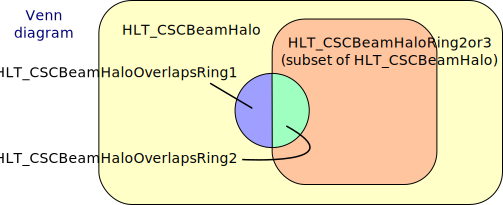
\includegraphics[width=0.85\linewidth]{venn_diagram.png}
\end{center}
\end{frame}

\begin{frame}
\frametitle{Rate needed for alignment}

\begin{itemize}
\item Track-based alignment performed with \textcolor{darkblue}{33,000} ring 1 overlaps  % 33,260 to be precise; only 10,440 in ring 2 (not enough to align twice as many chambers)
  events reaches desired accuracy (270~$\mu$m in the local $x$ direction) when
  compared with photogrammetry (an independent method)

\includegraphics[width=3.8 cm, angle=90]{compare_m31_x.pdf}
\includegraphics[height=3.8 cm]{delta_translations.pdf}

\item One complete alignment per day: \mbox{\textcolor{darkblue}{0.4~Hz} in \scriptsize HLT\_CSCBeamHaloOverlapsRing1\hspace{-3 cm}}

\item Ring 2 has twice as many chambers: needs \textcolor{darkblue}{0.8~Hz}

\item The above was actually collected in 9~minutes (60~Hz, no prescale)

\item Modest requirements: monitoring will mostly be important for keeping the rate low and well-distributed

\end{itemize}
\end{frame}

\begin{frame}
\frametitle{CSC beam-halo monitoring}

\begin{columns}
\column{0.6\linewidth}
\textcolor{darkblue}{Present:}
\begin{itemize}
\item L1 trigger rates and efficiencies in data
\item only HLT\_CSCBeamHalo path studied
\item version exists for release validation, but not regularly used
\end{itemize}

\column{0.4\linewidth}
\includegraphics[width=\linewidth]{TriggerOcc.png}

\textcolor{blue}{\mbox{\hspace{-1.4 cm}} \tt \tiny \href{http://tier2.ihepa.ufl.edu/~gartner/plots/Cosmics/}{http://tier2.ihepa.ufl.edu/$\sim$gartner/plots/Cosmics/}\mbox{\hspace{-2 cm}}}
\end{columns}

\vspace{0.5 cm}
\begin{columns}
\column{1.06\linewidth}
\textcolor{darkblue}{Future:}
\begin{itemize}
\item should track all four HLT paths
\item monitor continuous distributions, such as $x$-$y$ of CSC RecHits, to understand why the rate changes when it does
\item should be a routine part of RelVal, probably in DQM
\end{itemize}
\end{columns}
\end{frame}

\begin{frame}
\frametitle{Tracker-pointing cosmics plan}

\begin{itemize}
\item Needs trigger development before monitoring project begins
\begin{itemize}
\item no L1 emulator for RPC cosmics trigger yet (issue will be raised in Trigger Review on Wednesday)

\item current HLT implementation does full silicon tracking, but a
  standAloneMuon should be sufficient to determine if an RPC cosmic
  points to the tracker

\end{itemize}

\item Tracker DPG has named a responsible person and institution

\item \textcolor{darkblue}{Plan:} keep all 1--2~Hz of tracker-pointing
  cosmics, or if prescale is needed, make it $\phi$-dependent to reach
  sides of the detector

\end{itemize}

\vspace{0.5 cm}
\hspace{-0.83 cm} \textcolor{darkblue}{\Large Tracker beam-halo plan}

\vspace{0.1 cm}
\begin{itemize}
\item Seen as part of the same project/responsibility
\item Now that L1 emulator exists (recent development), only needs monitoring
\end{itemize}

%% \vspace{0.2 cm}
%% \hspace{-0.83 cm} \textcolor{darkblue}{\Large Tracker alignment minimum bias}

%% \vspace{0.05 cm}
%% \begin{itemize}
%% \item Plan to add a high-momentum ``minimum bias'' trigger with a lower prescale is preliminary
%% \end{itemize}

%% \vspace{0.2 cm}
%% \hspace{-0.83 cm} \textcolor{darkblue}{\Large Tracker LAS in the abort gap}

%% \vspace{0.05 cm}
%% \begin{itemize}
%% \item Preliminary planning
%% \end{itemize}
\end{frame}


%% \section*{First section}
%% \begin{frame}
%% \begin{center}
%% \Huge \textcolor{blue}{First section}
%% \end{center}
%% \end{frame}

\begin{frame}
\frametitle{Summary}

\begin{itemize}\setlength{\itemsep}{0.5 cm}
\item Status of all alignment-related triggers \mbox{given on pages~2--4\hspace{-1 cm}}
\item Reminder: most important events for alignment come from standard physics triggers--- single muon and minimum bias
\item Of the ``special'' triggers, brief status is
\begin{itemize}
\item CSC beam-halo: monitoring should be expanded
\item tracker cosmics: trigger development needed, monitoring will be a part of that
\item tracker beam-halo: only monitoring needed now
\item tracker considering extensions to minimum bias triggers
\item LAS planning to transfer data through the abort gap
\end{itemize}
\item Tracker DPG has named a person/institution responsible for cosmics and beam-halo (Yohann Tschudi, Lyon)
\end{itemize}

\label{numpages}
\end{frame}

\end{document}
